%=========================================================================
% sec-background
%=========================================================================

\section{Background}
\label{sec-background}

%=========================================================================
% fig-background-cnn.tex
%=========================================================================

\begin{figure}[h]

  \centering
  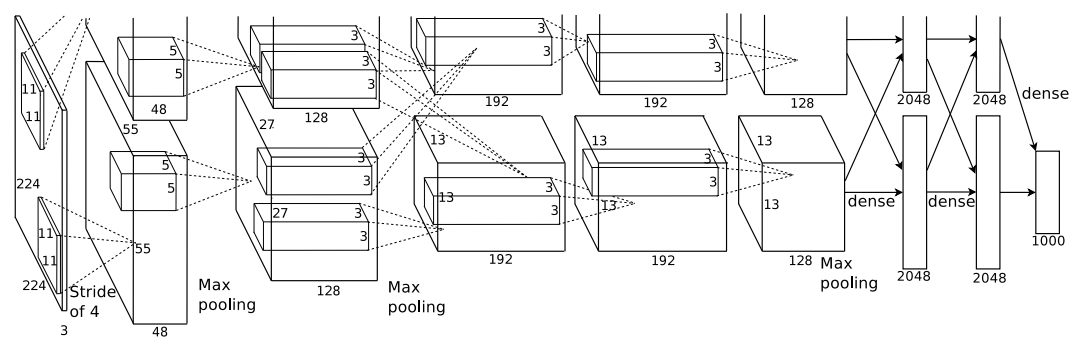
\includegraphics[width=0.9\tw]{fig-background-cnn.png}

  \caption{\textbf{Example CNN Pipeline --} The composition of layers in
    a CNN used for classifying images. A 224x244x3 (RGB-channels) input
    image is processed by five convolutional layers, two pooling layers,
    and two fully-connected layers to generate probabilities for 1000
    possible output labels. A. Krizhevsky, I. Sutskever,
    G. E. Hinton. ImageNet Classification with Deep Convolutional Neural
    Networks. NIPS 2012.}

  \label{fig-background-cnn}

\end{figure}


CNNs can be described as a pipeline of multiple computational layers,
where each layer applies a set of filters to the input to generate the
output that feeds into the next layer. Figure~\ref{fig-background-cnn}
shows an example CNN pipeline used by Krizhevsky and others in one of the
first successful attempts at accurate image classification. The types of
layers used in this example include the \emph{convolutional layer}, the
\emph{pooling layer}, and the \emph{fully connected layer}, and is
representative of the main types of layers used across all CNNs.

The convolutional layer takes a $X\times Y\times Z$ input and performs a 3D
convolution with $N$ $X'\times Y'\times Z$ filters to produce a
$X\times Y\times N$ output, where $X' < X, Y' < Y$. Each 3D convolution
with a unique filter generates one $X\times Y$ slice of the output. These
outputs are sometimes referred to as \emph{feature maps}. Each element in
the output also needs to be modified with a non-linear \emph{activation
  function}, such as tanh or ReLU.

The pooling layer downsamples a $X\times Y\times Z$ input using a
$M\times M$ window for each dimension in $Z$ to produce a
$(X/M)\times (Y/M)\times Z$ output. Downsampling is critical for capturing
a higher density of features in the feature map, but is not required
after every convolutional layer.

The layer types described above are examples of \emph{partially connected
  layers} where the elements of the output are only dependent of a subset
of input elements (e.g., the inputs used in the 3D convolution). In
contrast, each elements of the output in a fully connected layer is
dependent on \emph{all} of the input elements. Technically, this means
that a layer is fully connected if the filter dimensions match the input
dimensions. However, in practice, a fully connected layer generally has
one dimensional inputs and outputs, where an input of $N$ elements is
multiplied and reduced with $M$ filters of $N$ elements to produce an
output of $M$ elements. Fully connected layers are typically at the very
end of a CNN pipeline and are used to correlate feature maps to the
output labels.

As with any neural network, the accuracy of CNNs depends heavily on how
well the network is trained. Training may or may not be supervised, but
always involves exposing the network to a large number of labeled
instances to determine suitable \emph{weights} for the filters in each
layer. Training consists of \emph{forward propagation} and
\emph{backward propagation} phases. In the former, images with known
output labels are processed by the network to calculate the probabilities
that the input is classified as one of the possible output labels. In the
latter, the delta between the empirically classified label and the
correct label is used to perform a gradient descent with which to update
the weights in the CNNs. These phases are repeated as many times as
needed to determine the weights that minimize the \emph{loss function}
that describes the error rate for classifying the inputs.
